% Enhanced 3D U-Net Architecture Figure with Attention Gate Inset
% Compile with: pdflatex enhanced_unet_with_inset.tex

\documentclass{article}
\usepackage[paperwidth=32cm, paperheight=14cm, margin=0.5cm]{geometry}
\usepackage{tikz}
\usepackage{xcolor}
\usepackage{amsmath}

\usetikzlibrary{shapes.geometric, arrows.meta, positioning, calc, backgrounds, fit, decorations.pathreplacing}

% Define colors (colorblind-friendly palette)
\definecolor{encoderblue}{RGB}{55, 126, 184}
\definecolor{decodergreen}{RGB}{77, 175, 74}
\definecolor{bottleneckorange}{RGB}{255, 127, 0}
\definecolor{attentionpurple}{RGB}{152, 78, 163}
\definecolor{skipgray}{RGB}{100, 100, 100}
\definecolor{dsred}{RGB}{228, 26, 28}
\definecolor{inputgray}{RGB}{200, 200, 200}

\pagestyle{empty}

\begin{document}
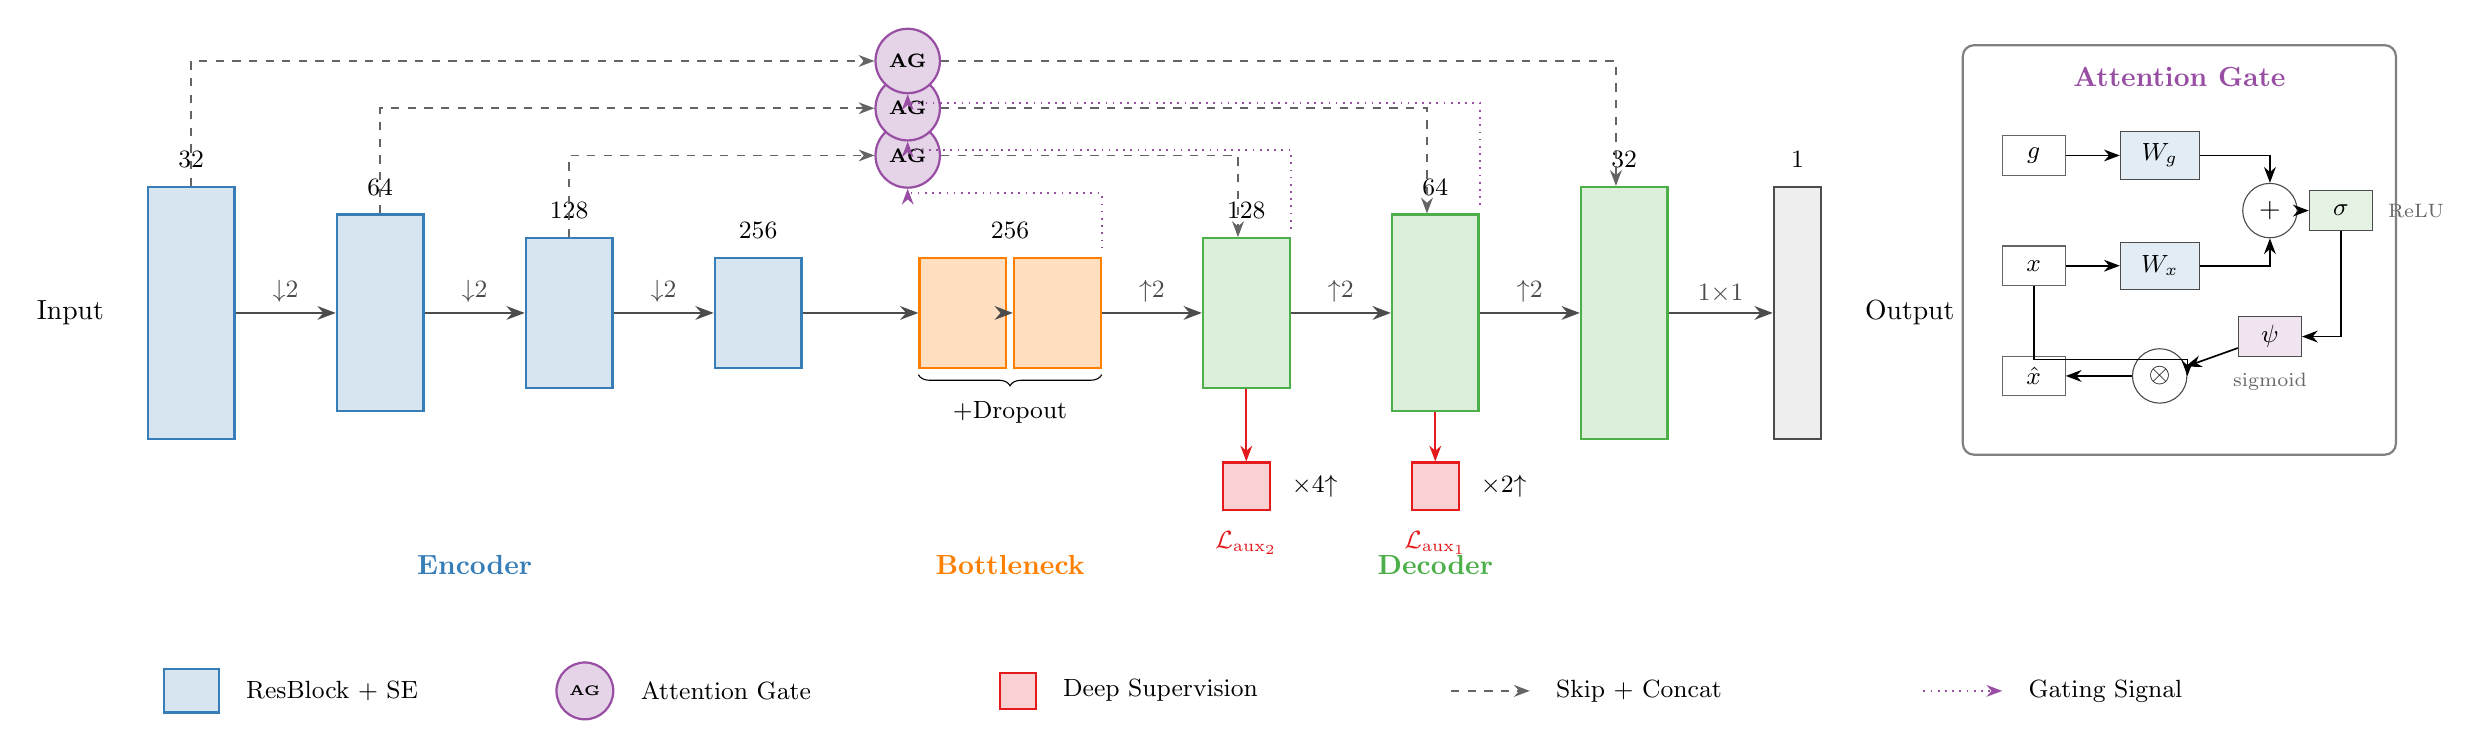
\begin{tikzpicture}[
    % Encoder block
    enc/.style={
        rectangle,
        draw=encoderblue,
        fill=encoderblue!20,
        line width=0.8pt,
        minimum width=1.1cm,
    },
    % Decoder block
    dec/.style={
        rectangle,
        draw=decodergreen,
        fill=decodergreen!20,
        line width=0.8pt,
        minimum width=1.1cm,
    },
    % Bottleneck block
    bottle/.style={
        rectangle,
        draw=bottleneckorange,
        fill=bottleneckorange!25,
        line width=0.8pt,
        minimum width=1.1cm,
    },
    % Attention gate
    attgate/.style={
        circle,
        draw=attentionpurple,
        fill=attentionpurple!25,
        line width=0.8pt,
        minimum size=0.7cm,
        font=\small\bfseries,
    },
    % Deep supervision
    dsblock/.style={
        rectangle,
        draw=dsred,
        fill=dsred!20,
        line width=0.8pt,
        minimum width=0.6cm,
        minimum height=0.6cm,
        font=\scriptsize,
    },
    % Output block
    outblock/.style={
        rectangle,
        draw=black!70,
        fill=inputgray!30,
        line width=0.8pt,
        minimum width=0.6cm,
    },
    % Arrow styles
    flow/.style={->, >=Stealth, thick, black!70},
    skip/.style={->, >=Stealth, semithick, skipgray, dashed},
    gate/.style={->, >=Stealth, semithick, attentionpurple, dotted},
    dsarrow/.style={->, >=Stealth, semithick, dsred},
    % Labels
    chanlabel/.style={font=\small, above=3pt},
    sublabel/.style={font=\tiny, text=black!60},
]

% =====================================================
% MAIN ARCHITECTURE - Increased horizontal spacing
% =====================================================

% Encoder blocks (heights represent spatial dimensions)
\node[enc, minimum height=3.2cm] (e0) at (0, 0) {};
\node[enc, minimum height=2.5cm] (e1) at (2.4, 0) {};
\node[enc, minimum height=1.9cm] (e2) at (4.8, 0) {};
\node[enc, minimum height=1.4cm] (e3) at (7.2, 0) {};

% Channel labels - more space above
\node[chanlabel] at (e0.north) {32};
\node[chanlabel] at (e1.north) {64};
\node[chanlabel] at (e2.north) {128};
\node[chanlabel] at (e3.north) {256};

% Bottleneck (two blocks) - more space between
\node[bottle, minimum height=1.4cm] (b1) at (9.8, 0) {};
\node[bottle, minimum height=1.4cm] (b2) at (11.0, 0) {};
\node[chanlabel] at ($(b1.north)!0.5!(b2.north)$) {256};

% Dropout indicator
\draw[decorate, decoration={brace, amplitude=4pt, mirror}]
    ([yshift=-2pt]b1.south west) -- ([yshift=-2pt]b2.south east)
    node[midway, below=6pt, font=\small] {+Dropout};

% Decoder blocks - increased spacing
\node[dec, minimum height=1.9cm] (d2) at (13.4, 0) {};
\node[dec, minimum height=2.5cm] (d1) at (15.8, 0) {};
\node[dec, minimum height=3.2cm] (d0) at (18.2, 0) {};

\node[chanlabel] at (d2.north) {128};
\node[chanlabel] at (d1.north) {64};
\node[chanlabel] at (d0.north) {32};

% Output
\node[outblock, minimum height=3.2cm] (out) at (20.4, 0) {};
\node[chanlabel] at (out.north) {1};

% =====================================================
% MAIN FLOW ARROWS
% =====================================================

% Encoder path
\draw[flow] (e0.east) -- (e1.west) node[midway, above, font=\small] {$\downarrow$2};
\draw[flow] (e1.east) -- (e2.west) node[midway, above, font=\small] {$\downarrow$2};
\draw[flow] (e2.east) -- (e3.west) node[midway, above, font=\small] {$\downarrow$2};
\draw[flow] (e3.east) -- (b1.west);
\draw[flow] (b1.east) -- (b2.west);

% Decoder path
\draw[flow] (b2.east) -- (d2.west) node[midway, above, font=\small] {$\uparrow$2};
\draw[flow] (d2.east) -- (d1.west) node[midway, above, font=\small] {$\uparrow$2};
\draw[flow] (d1.east) -- (d0.west) node[midway, above, font=\small] {$\uparrow$2};
\draw[flow] (d0.east) -- (out.west) node[midway, above, font=\small] {1$\times$1};

% =====================================================
% ATTENTION GATES AND SKIP CONNECTIONS - More vertical space
% =====================================================

% Attention gate nodes - staggered higher
\node[attgate] (ag2) at ($(e2)!0.5!(d2) + (0, 2.0)$) {\scriptsize AG};
\node[attgate] (ag1) at ($(e1)!0.5!(d1) + (0, 2.6)$) {\scriptsize AG};
\node[attgate] (ag0) at ($(e0)!0.5!(d0) + (0, 3.2)$) {\scriptsize AG};

% Skip connections: encoder -> attention gate
\draw[skip] (e2.north) |- (ag2.west);
\draw[skip] (e1.north) |- (ag1.west);
\draw[skip] (e0.north) |- (ag0.west);

% Attention gate -> decoder (concatenation point)
\draw[skip] (ag2.east) -| ([xshift=-3pt]d2.north);
\draw[skip] (ag1.east) -| ([xshift=-3pt]d1.north);
\draw[skip] (ag0.east) -| ([xshift=-3pt]d0.north);

% Gating signals (from decoder path to attention gates)
\draw[gate] ([yshift=3pt]b2.north east) -- ++(0, 0.7) -| (ag2.south);
\draw[gate] ([yshift=3pt]d2.north east) -- ++(0, 1.0) -| (ag1.south);
\draw[gate] ([yshift=3pt]d1.north east) -- ++(0, 1.3) -| (ag0.south);

% =====================================================
% DEEP SUPERVISION - More space below
% =====================================================

\node[dsblock] (ds2) at (13.4, -2.2) {};
\node[dsblock] (ds1) at (15.8, -2.2) {};

\draw[dsarrow] (d2.south) -- (ds2.north);
\draw[dsarrow] (d1.south) -- (ds1.north);

\node[below=4pt of ds2, font=\small, dsred] {$\mathcal{L}_{\text{aux}_2}$};
\node[below=4pt of ds1, font=\small, dsred] {$\mathcal{L}_{\text{aux}_1}$};
\node[right=4pt of ds2, font=\small] {$\times$4$\uparrow$};
\node[right=4pt of ds1, font=\small] {$\times$2$\uparrow$};

% =====================================================
% INPUT/OUTPUT LABELS
% =====================================================

\node[left=12pt of e0, font=\normalsize] {Input};
\node[right=12pt of out, font=\normalsize] {Output};

% Section labels - more space below
\node[font=\normalsize\bfseries, encoderblue] at (3.6, -3.2) {Encoder};
\node[font=\normalsize\bfseries, bottleneckorange] at (10.4, -3.2) {Bottleneck};
\node[font=\normalsize\bfseries, decodergreen] at (15.8, -3.2) {Decoder};

% =====================================================
% ATTENTION GATE INSET - More space, larger elements
% =====================================================

\begin{scope}[shift={(23.0, 1.2)}, scale=1.0]
    % Inset box - larger
    \draw[black!50, thick, rounded corners=4pt] (-0.5, -3.0) rectangle (5.0, 2.2);
    \node[font=\normalsize\bfseries, attentionpurple] at (2.25, 1.8) {Attention Gate};

    % Gate signal input
    \node[rectangle, draw=black!60, fill=white, minimum width=0.8cm, minimum height=0.5cm, font=\small] (g_in) at (0.4, 0.8) {$g$};

    % Skip input
    \node[rectangle, draw=black!60, fill=white, minimum width=0.8cm, minimum height=0.5cm, font=\small] (x_in) at (0.4, -0.6) {$x$};

    % W_g transform
    \node[rectangle, draw=black!70, fill=encoderblue!15, minimum width=1.0cm, minimum height=0.6cm, font=\small] (wg) at (2.0, 0.8) {$W_g$};

    % W_x transform
    \node[rectangle, draw=black!70, fill=encoderblue!15, minimum width=1.0cm, minimum height=0.6cm, font=\small] (wx) at (2.0, -0.6) {$W_x$};

    % Addition
    \node[circle, draw=black!70, fill=white, minimum size=0.55cm, font=\normalsize] (add) at (3.4, 0.1) {$+$};

    % ReLU
    \node[rectangle, draw=black!70, fill=decodergreen!15, minimum width=0.8cm, minimum height=0.5cm, font=\small] (relu) at (4.3, 0.1) {$\sigma$};

    % Psi (1x1 conv + sigmoid)
    \node[rectangle, draw=black!70, fill=attentionpurple!15, minimum width=0.8cm, minimum height=0.5cm, font=\small] (psi) at (3.4, -1.5) {$\psi$};

    % Multiplication
    \node[circle, draw=black!70, fill=white, minimum size=0.55cm, font=\normalsize] (mul) at (2.0, -2.0) {$\otimes$};

    % Output
    \node[rectangle, draw=black!60, fill=white, minimum width=0.8cm, minimum height=0.5cm, font=\small] (out_ag) at (0.4, -2.0) {$\hat{x}$};

    % Arrows
    \draw[->, >=Stealth, semithick] (g_in) -- (wg);
    \draw[->, >=Stealth, semithick] (x_in) -- (wx);
    \draw[->, >=Stealth, semithick] (wg) -| (add);
    \draw[->, >=Stealth, semithick] (wx) -| (add);
    \draw[->, >=Stealth, semithick] (add) -- (relu);
    \draw[->, >=Stealth, semithick] (relu) |- (psi);
    \draw[->, >=Stealth, semithick] (psi) -- (mul);
    \draw[->, >=Stealth, semithick] (mul) -- (out_ag);
    \draw[->, >=Stealth, semithick] (x_in) |- ([yshift=6pt]mul.east) -- (mul.east);

    % Labels
    \node[font=\scriptsize, text=black!60, below=2pt of psi] {sigmoid};
    \node[font=\scriptsize, text=black!60, right=2pt of relu] {ReLU};
\end{scope}

% =====================================================
% LEGEND - More spacing between items
% =====================================================

\begin{scope}[shift={(0, -4.8)}]
    % ResBlock + SE
    \node[enc, minimum height=0.55cm, minimum width=0.7cm] (l1) at (0, 0) {};
    \node[font=\small, right=6pt of l1] {ResBlock + SE};

    % Attention Gate
    \node[attgate, minimum size=0.5cm] (l2) at (5.0, 0) {\tiny AG};
    \node[font=\small, right=6pt of l2] {Attention Gate};

    % Deep Supervision
    \node[dsblock, minimum height=0.45cm, minimum width=0.45cm] (l3) at (10.5, 0) {};
    \node[font=\small, right=6pt of l3] {Deep Supervision};

    % Skip connection
    \draw[skip] (16.0, 0) -- ++(1.0, 0);
    \node[font=\small, right=6pt] at (17.0, 0) {Skip + Concat};

    % Gating signal
    \draw[gate] (22.0, 0) -- ++(1.0, 0);
    \node[font=\small, right=6pt] at (23.0, 0) {Gating Signal};
\end{scope}

\end{tikzpicture}
\end{document}
